\documentclass{article}

\title{	
	\normalfont\normalsize 
	\rule{\linewidth}{0.5pt}\\ % Thin top horizontal rule
	\vspace{14pt} % Whitespace
	{\LARGE MATH401 Assignment 2 \\ % The assignment title
    \large \textit{} \\}
	\vspace{6pt} % Whitespace
	\rule{\linewidth}{1pt}\\ % Thick bottom horizontal rule
}

\author{Elliott Hughes}
\date{\normalsize\today}
\usepackage{tikz}
\usetikzlibrary{arrows,automata}
\usetikzlibrary{positioning}
\usetikzlibrary{arrows.meta,positioning}
\usepackage{mdframed}
\usepackage{amsmath}
\usepackage{amssymb}
\usepackage{graphicx}
\graphicspath{ {./Images/Assignment_2/} }
\usepackage{commath}
\usepackage{textcomp}
\usepackage{gensymb}
\usepackage{float}
\usepackage{hyperref}
\usepackage[margin=1in]{geometry}
\usepackage{caption}
\usepackage{subcaption}
\usepackage{sectsty}
\usepackage{titlesec}

\begin{document}

\maketitle

\subsection*{Q28}
Suppose that $A$ is a $2\times 2$ matrix with eigenvalues $\lambda_1,\, \lambda_2$ and 
corresponding eigenvectors $v_1$ and $v_2$. Furthermore 
let us assume that $|\lambda_1| = 1$ and $\lambda_2 \in \mathbb{C}$. Consider the dynamical 
system $f^n(x) = A^nx$. By definition $v_1 \notin span\{v_2\}$ so for some $x \in \mathbb{R}^2$ 
we can write $x = av_1 + bv_2$ for some $a,b \in \mathbb{R}$. By the linearity of matrices we can 
then decompose the action of this system $f^n(x) = A^nx = \lambda_1^nav_1 + \lambda_2^nbv_2$.

\paragraph{Subcase 1.1}
Consider the possible options for $\lambda_1$. If $\lambda_1 = 1$ then the first term is 
simply $av_1$. This also implies that $\lambda_2 \in \mathbb{R}$ since our map is from the reals to 
the reals. If $|\lambda_2| < 1$ this implies that the second term approaches zero 
in the limit. Therefore all points will approach the the line $span\{v_1\}$ in the limit, 
so this is a line of attracting fixed points. \autoref{fig:subcase1.1} provides a sketch 
example of such a system (note that all sketches within this section show only the simplest 
possible cases of such systems and more complex dynamics with similar limiting behavior are 
possible).

\begin{figure}[H]
	\centering
	\begin{tikzpicture}[point/.style={circle, very thick, draw=black!60,inner sep = 0.3mm}]
		\draw (3,0) -- (-3,0);
		\node[point] at (1,3) {};
		\node[point] at (-1,3) {};
		\node[point] at (1,2) {};
		\node[point] at (-1,2) {};
		\node[point] at (-1,1) {};
		\node[point] at (1,1) {};
		\draw[->] (-1,2.9) -- (-1,2.1);
		\draw[->] (1,2.9) -- (1,2.1);
		\draw[->] (-1,1.9) -- (-1,1.1);
		\draw[->] (1,1.9) -- (1,1.1);

		\node[point] at (1,-3) {};
		\node[point] at (-1,-3) {};
		\node[point] at (1,-2) {};
		\node[point] at (-1,-2) {};
		\node[point] at (-1,-1) {};
		\node[point] at (1,-1) {};
		\draw[->] (-1,-2.9) -- (-1,-2.1);
		\draw[->] (1,-2.9) -- (1,-2.1);
		\draw[->] (-1,-1.9) -- (-1,-1.1);
		\draw[->] (1,-1.9) -- (1,-1.1);

		\node at (1,1.5) [label = left:$A$] {};
		\node at (1,2.5) [label = left:$A$] {};
		\node at (-1,1.5) [label = left:$A$] {};
		\node at (-1,2.5) [label = left:$A$] {};
		
		\node at (1,-1.5) [label = left:$A$] {};
		\node at (1,-2.5) [label = left:$A$] {};
		\node at (-1,-1.5) [label = left:$A$] {};
		\node at (-1,-2.5) [label = left:$A$] {};

		\node at (3,0) [label = right:$v_1$] {};
	\end{tikzpicture}
	\caption{A prototypical system with $\lambda_1 = 1$ and $|\lambda_2| < 1$. In the limit, 
	points approach their projection in the subspace defined by the span of $v_1$.}
	\label{fig:subcase1.1}
\end{figure}

\paragraph{Subcase 1.2 and 1.3}
If $|\lambda_2| = 1$ then either $\lambda_2 = 1$ or $\lambda_2 = -1$. If $\lambda_2 = 1$ then 
this map is the identity map and so $A^nx = x$. If $\lambda_2 = -1$ then clearly the system 
will flip points about the line formed by the span of $v_1$ (see \autoref{fig:subcase1.3} for a 
stylized sketch of the situation). This suggests that points on the line are fixed and all other 
points have period two.

\begin{figure}[H]
	\centering
	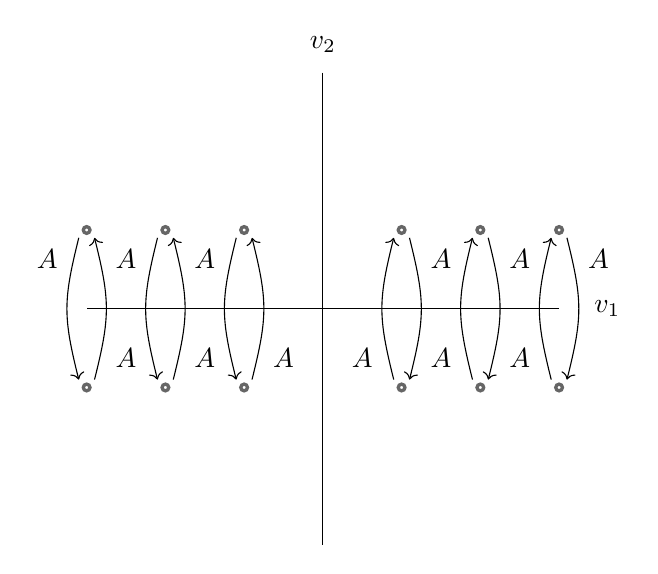
\begin{tikzpicture}[point/.style={circle, very thick, draw=black!60,inner sep = 0.3mm}]
		\draw (3,0) -- (-3,0);
		\draw (0,3) -- (0,-3);
		\node[point] at (3,1) {};
		\node[point] at (3,-1) {};
		\node[point] at (2,1) {};
		\node[point] at (2,-1) {};
		\node[point] at (1,-1) {};
		\node[point] at (1,1) {};
		\node[point] at (-3,1) {};
		\node[point] at (-3,-1) {};
		\node[point] at (-2,1) {};
		\node[point] at (-2,-1) {};
		\node[point] at (-1,-1) {};
		\node[point] at (-1,1) {};

		\draw[->] (2.9,-0.9) .. controls (2.7,-0.1) and (2.7,0.1) ..  (2.9,0.9);
		\draw[->] (1.9,-0.9) .. controls (1.7,-0.1) and (1.7,0.1) .. (1.9,0.9);
		\draw[->] (0.9,-0.9) .. controls (0.7,-0.1) and (0.7,0.1) .. (0.9,0.9);
		\draw[<-] (3.1,-0.9) .. controls (3.3,-0.1) and (3.3,0.1) ..  (3.1,0.9);
		\draw[<-] (2.1,-0.9) .. controls (2.3,-0.1) and (2.3,0.1) .. (2.1,0.9);
		\draw[<-] (1.1,-0.9) .. controls (1.3,-0.1) and (1.3,0.1) .. (1.1,0.9);

		\draw[->] (-2.9,-0.9) .. controls (-2.7,-0.1) and (-2.7,0.1) .. (-2.9,0.9);
		\draw[->] (-1.9,-0.9) .. controls (-1.7,-0.1) and (-1.7,0.1) .. (-1.9,0.9);
		\draw[->] (-0.9,-0.9) .. controls (-0.7,-0.1) and (-0.7,0.1) .. (-0.9,0.9);
		\draw[<-] (-3.1,-0.9) .. controls (-3.3,-0.1) and (-3.3,0.1) .. (-3.1,0.9);
		\draw[<-] (-2.1,-0.9) .. controls (-2.3,-0.1) and (-2.3,0.1) .. (-2.1,0.9);
		\draw[<-] (-1.1,-0.9) .. controls (-1.3,-0.1) and (-1.3,0.1) .. (-1.1,0.9);

		\node at (1.5,1) [label = below:$A$] {};
		\node at (2.5,1) [label = below:$A$] {};
		\node at (3.5,1) [label = below:$A$] {};

		\node at (1.5,-1) [label = above:$A$] {};
		\node at (2.5,-1) [label = above:$A$] {};
		\node at (0.5,-1) [label = above:$A$] {};
		

		\node at (-1.5,1) [label = below:$A$] {};
		\node at (-2.5,1) [label = below:$A$] {};
		\node at (-3.5,1) [label = below:$A$] {};
		
		\node at (-1.5,-1) [label = above:$A$] {};
		\node at (-2.5,-1) [label = above:$A$] {};
		\node at (-0.5,-1) [label = above:$A$] {};

		\node at (0,3) [label = above:$v_2$] {};
		\node at (3.2,0) [label = right:$v_1$] {};
	\end{tikzpicture}
	\caption{A prototypical system with $\lambda_1 = 1$ and $\lambda_2 = -1$. Points are reflected 
	across the line defined by the span of $v_1$.}
	\label{fig:subcase1.3}
\end{figure}

\paragraph{Subcase 1.4}
If $|\lambda_2| > 1$ then clearly all points not on the span of $v_1$ will leave the neighborhood of this line. In fact, since 
the matrix $A$ has full rank in this case, we can define the inverse $A^{-1}$. This matrix will 
have the same eigenvectors with corresponding eigenvalues $\rho_i = 1/\lambda_i$ and so the system 
$f^{-n}(x) = A^{-n}x$ is the same as subcase $1.1$ above. Therefore the line $span\{v_1\}$ is a 
line of repelling fixed points (see \autoref{fig:subcase1.4}).

\begin{figure}[H]
	\centering
	\begin{tikzpicture}[point/.style={circle, very thick, draw=black!60,inner sep = 0.3mm}]
		\draw (3,0) -- (-3,0);
		\node[point] at (1,3) {};
		\node[point] at (-1,3) {};
		\node[point] at (1,2) {};
		\node[point] at (-1,2) {};
		\node[point] at (-1,1) {};
		\node[point] at (1,1) {};
		\draw[<-] (-1,2.9) -- (-1,2.1);
		\draw[<-] (1,2.9) -- (1,2.1);
		\draw[<-] (-1,1.9) -- (-1,1.1);
		\draw[<-] (1,1.9) -- (1,1.1);

		\node[point] at (1,-3) {};
		\node[point] at (-1,-3) {};
		\node[point] at (1,-2) {};
		\node[point] at (-1,-2) {};
		\node[point] at (-1,-1) {};
		\node[point] at (1,-1) {};
		\draw[<-] (-1,-2.9) -- (-1,-2.1);
		\draw[<-] (1,-2.9) -- (1,-2.1);
		\draw[<-] (-1,-1.9) -- (-1,-1.1);
		\draw[<-] (1,-1.9) -- (1,-1.1);

		\node at (1,1.5) [label = left:$A$] {};
		\node at (1,2.5) [label = left:$A$] {};
		\node at (-1,1.5) [label = left:$A$] {};
		\node at (-1,2.5) [label = left:$A$] {};
		
		\node at (1,-1.5) [label = left:$A$] {};
		\node at (1,-2.5) [label = left:$A$] {};
		\node at (-1,-1.5) [label = left:$A$] {};
		\node at (-1,-2.5) [label = left:$A$] {};

		\node at (3,0) [label = right:$v_1$] {};
	\end{tikzpicture}
	\caption{A prototypical system with $\lambda_1 = 1$ and $|\lambda_2| > 1$. Points move orthogonally 
	away from the line defined by the span of $v_1$.}
	\label{fig:subcase1.4}
\end{figure}

\paragraph{Case 2}
If $\lambda_1 = -1$ then the map will reflect points across the line formed by the span of $v_2$. 
In general there are three cases to consider; $|\lambda_2| < 1$, $\lambda_2 = -1$ or $|\lambda_2| > 1$ (if $|\lambda_2| =1$ 
then this is simply Subcase 1.2 above).

\paragraph{Case 2.1}
If $|\lambda_2| < 1$ then points will approach the line $span\{v_1\}$, but the points on this 
line are not fixed. Nonetheless this line remains fixed under the action of $A$ (\autoref{fig:subcase2.1}) 
and all points on this line have period two. 

\begin{figure}[H]
	\centering
	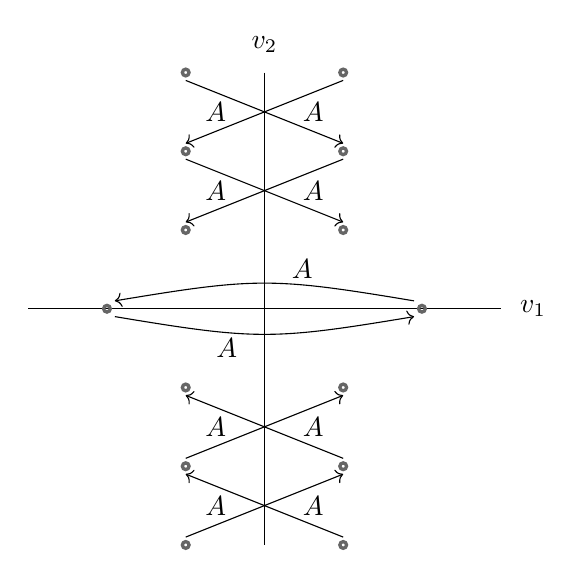
\begin{tikzpicture}[point/.style={circle, very thick, draw=black!60,inner sep = 0.3mm}]
		\draw (0,3) -- (0,-3);
		\draw (3,0) -- (-3,0);
		\node[point] at (1,3) {};
		\node[point] at (-1,3) {};
		\node[point] at (1,2) {};
		\node[point] at (-1,2) {};
		\node[point] at (-1,1) {};
		\node[point] at (1,1) {};
		\draw[->] (-1,2.9) -- (1,2.1);
		\draw[->] (1,2.9) -- (-1,2.1);
		\draw[->] (-1,1.9) -- (1,1.1);
		\draw[->] (1,1.9) -- (-1,1.1);

		\node[point] at (1,-3) {};
		\node[point] at (-1,-3) {};
		\node[point] at (1,-2) {};
		\node[point] at (-1,-2) {};
		\node[point] at (-1,-1) {};
		\node[point] at (1,-1) {};
		\draw[->] (-1,-2.9) -- (1,-2.1);
		\draw[->] (1,-2.9) -- (-1,-2.1);
		\draw[->] (-1,-1.9) -- (1,-1.1);
		\draw[->] (1,-1.9) -- (-1,-1.1);

		\node at (1,1.5) [label = left:$A$] {};
		\node at (1,2.5) [label = left:$A$] {};
		\node at (-1,1.5) [label = right:$A$] {};
		\node at (-1,2.5) [label = right:$A$] {};
		
		\node at (1,-1.5) [label = left:$A$] {};
		\node at (1,-2.5) [label = left:$A$] {};
		\node at (-1,-1.5) [label = right:$A$] {};
		\node at (-1,-2.5) [label = right:$A$] {};

		\node[point] at (2,0) {};
		\node[point] at (-2,0) {};
		\draw[->] (1.9,0.1) .. controls (0.1,0.4) and (-0.1,0.4) .. (-1.9,0.1);
		\draw[<-] (1.9,-0.1) .. controls (0.1,-0.4) and (-0.1,-0.4) .. (-1.9,-0.1);
		\node at (0.1,0.5) [label = right:$A$] {};
		\node at (-0.1,-0.5) [label = left:$A$] {};
		


		\node at (0,3) [label = above:$v_2$] {};
		\node at (3,0) [label = right:$v_1$] {};
	\end{tikzpicture}
	\caption{A prototypical system with $\lambda_1 = -1$ and $|\lambda_2| < 1$. In the limit, 
	points approach the line defined by the span of $v_1$, but points on this line are not fixed under the 
	map.}
	\label{fig:subcase2.1}
\end{figure}

\paragraph{Case 2.2}
If $\lambda_1 = \lambda_2 = -1$ then this map reflects points about the lines formed by the 
span of each eigenvector (\autoref{fig:subcase2.2}). Consequently all points have period two.

\begin{figure}[H]
	\centering
	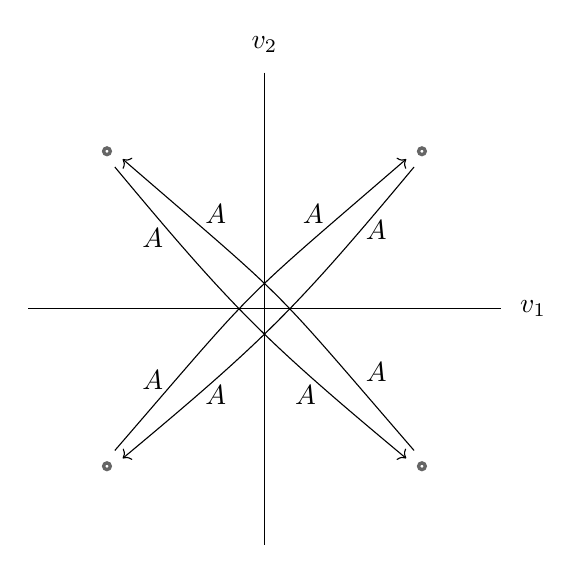
\begin{tikzpicture}[point/.style={circle, very thick, draw=black!60,inner sep = 0.3mm}]
		\draw (0,3) -- (0,-3);
		\draw (3,0) -- (-3,0);
		\node[point] at (2,2) {};
		\node[point] at (-2,2) {};
		\node[point] at (2,-2) {};
		\node[point] at (-2,-2) {};
		
		\draw[->] (1.9,1.8) .. controls (0.4,0) and (0,-0.4).. (-1.8,-1.9);
		\draw[->] (-1.9,1.8) .. controls (-0.4,0) and (0,-0.4).. (1.8,-1.9);
		\draw[<-] (1.8,1.9) .. controls (-0.4,0) and (0,0.4).. (-1.9,-1.8);
		\draw[<-] (-1.8,1.9) .. controls (0.4,0) and (0,0.4).. (1.9,-1.8);


		\node at (1,1.2) [label = left:$A$] {};
		\node at (1.8,1) [label = left:$A$] {};
		\node at (-1,1.2) [label = right:$A$] {};
		\node at (1.8,-0.8) [label = left:$A$] {};
		
		\node at (-1.8,0.9) [label = right:$A$] {};
		\node at (0.9,-1.1) [label = left:$A$] {};
		\node at (-1,-1.1) [label = right:$A$] {};
		\node at (-1.8,-0.9) [label = right:$A$] {};



		\node at (0,3) [label = above:$v_2$] {};
		\node at (3,0) [label = right:$v_1$] {};
	\end{tikzpicture}
	\caption{A prototypical system with $\lambda_1 = -1$ and $\lambda_2 = -1$. The lines 
	generated the span of each eigenvector remain fixed, but points are reflected across both lines.}
	\label{fig:subcase2.2}
\end{figure}

\paragraph{Case 2.3}
If $|\lambda_2| > 1$ then the line $span\{v_1\}$ remains fixed, but points near this line approach 
do not stay near this point and instead diverge in modulus to infinity as $n \rightarrow \infty$ (\autoref{fig:subcase2.3}).


\begin{figure}[H]
	\centering
	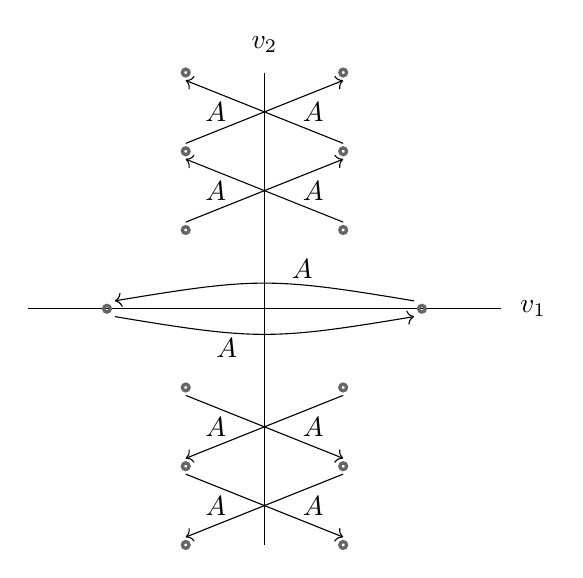
\begin{tikzpicture}[point/.style={circle, very thick, draw=black!60,inner sep = 0.3mm}]
		\draw (0,3) -- (0,-3);
		\draw (3,0) -- (-3,0);
		\node[point] at (1,3) {};
		\node[point] at (-1,3) {};
		\node[point] at (1,2) {};
		\node[point] at (-1,2) {};
		\node[point] at (-1,1) {};
		\node[point] at (1,1) {};
		\draw[<-] (-1,2.9) -- (1,2.1);
		\draw[<-] (1,2.9) -- (-1,2.1);
		\draw[<-] (-1,1.9) -- (1,1.1);
		\draw[<-] (1,1.9) -- (-1,1.1);

		\node[point] at (1,-3) {};
		\node[point] at (-1,-3) {};
		\node[point] at (1,-2) {};
		\node[point] at (-1,-2) {};
		\node[point] at (-1,-1) {};
		\node[point] at (1,-1) {};
		\draw[<-] (-1,-2.9) -- (1,-2.1);
		\draw[<-] (1,-2.9) -- (-1,-2.1);
		\draw[<-] (-1,-1.9) -- (1,-1.1);
		\draw[<-] (1,-1.9) -- (-1,-1.1);

		\node at (1,1.5) [label = left:$A$] {};
		\node at (1,2.5) [label = left:$A$] {};
		\node at (-1,1.5) [label = right:$A$] {};
		\node at (-1,2.5) [label = right:$A$] {};
		
		\node at (1,-1.5) [label = left:$A$] {};
		\node at (1,-2.5) [label = left:$A$] {};
		\node at (-1,-1.5) [label = right:$A$] {};
		\node at (-1,-2.5) [label = right:$A$] {};

		\node[point] at (2,0) {};
		\node[point] at (-2,0) {};
		\draw[->] (1.9,0.1) .. controls (0.1,0.4) and (-0.1,0.4) .. (-1.9,0.1);
		\draw[<-] (1.9,-0.1) .. controls (0.1,-0.4) and (-0.1,-0.4) .. (-1.9,-0.1);
		\node at (0.1,0.5) [label = right:$A$] {};
		\node at (-0.1,-0.5) [label = left:$A$] {};
		


		\node at (0,3) [label = above:$v_2$] {};
		\node at (3,0) [label = right:$v_1$] {};
	\end{tikzpicture}
	\caption{A prototypical system with $\lambda_1 = -1$ and $|\lambda_2| > 1$. Points not on the 
	line defined by the span of $v_1$ depart its neighborhood. The line itself remains fixed, but 
	points on this line are reflected about the origin.}
	\label{fig:subcase2.3}
\end{figure}

\paragraph{Case 3}
If $|\lambda_1| = 1$ and $\lambda_1 \in \mathbb{R}\backslash \mathbb{C}$ then $\lambda_2 = \overline{\lambda_1}$ 
since this matrix is from $\mathbb{R}^2$ to $\mathbb{R}^2$. For a matrix from $\mathbb{R}^2$ to 
$\mathbb{R}^2$ it is possible to decompose a matrix $A$ into a product of $C$, $C^{-1}$ and 
$B$ where $B$ is a rotation-scaling matrix. In particular, if $v_1 = z + iw$ then $C = [z,w]$ 
and if $\lambda_1 = a + bi$ then 

\begin{equation*}
	B = 
	\begin{bmatrix}
		a & -b \\ b & a
	\end{bmatrix}
\end{equation*}

A sketch of the proof follows. First it is necessary to show that $C$ is invertible, so that 
this equation is well-defined. To introduce a contradiction we assume that there exists $\gamma,\xi \in \mathbb{R}$ such that 
$\xi z + \gamma w = 0$. Then this implies that $v_* = (\xi + i\gamma)v_1 = \gamma z - \xi w + i(\xi z + \gamma w)$. 
This is an eigenvector with corresponding eigenvalue $\lambda_1$. But clearly this is real by 
our previous assumption, so $Av_* \notin \mathbb{C}^2\backslash\mathbb{R}^2$ and we obtain a contradiction. Thus 
$C$ must be invertible. It remains to show that this decomposition is correct. By direct 
computation we can see that 

\begin{equation*}
	Av_1 = \lambda_1v_1 = (a+bi)
	\begin{bmatrix}
		z_1 + iw_1 \\ z_2 + iw_2
	\end{bmatrix}
	=
	\begin{bmatrix}
		az_1-bw_1 \\ az_2 - bw_2
	\end{bmatrix}
	+ i
	\begin{bmatrix}
		aw_1 + bz_1 \\ aw_2 + bz_2
	\end{bmatrix}
\end{equation*}

Where $z = (z_1,z_2)$ and $w = (w_1,w_2)$. Furthermore it is also clear that

\begin{equation*}
	A\left(
		\begin{bmatrix}
			z_1 \\ z_2
		\end{bmatrix}
		+ i
		\begin{bmatrix}
			w_1 \\ w_2
		\end{bmatrix}
	\right)
	= 
	Az + iAw
\end{equation*}

Equating real and imaginary parts this suggests that 

\begin{equation*}
	Az = 
	\begin{bmatrix}
		az_1-bw_1 \\ az_2 - bw_2
	\end{bmatrix}
	\qquad 
	Aw = 
	\begin{bmatrix}
		aw_1 + bz_1 \\ aw_2 + bz_2
	\end{bmatrix}
\end{equation*}

It is then straightforward to compute the action of $CBC^{-1}$ on these vectors and note that 
they are mapped to the same location by both matrices. Since these vectors are linearly independent 
it follows that $A$ and $CBC^{-1}$ act the same on all vectors in $\mathbb{R}^2$ and consequently 
that $A = CBC^{-1}$.

\paragraph{}
Since the eigenvalues of the matrix have modulus one in this case, the rotation scaling matrix 
is simply a rotation matrix. Therefore the iterated action of this map is simply $A^nx = CB^nC^{-1}x$. 
So the action of this map is simply a change of basis vectors, rotation in this space and then a 
basis change back to the original basis. Then if we write $a+bi=\cos(\theta) + i\sin(\theta)$ 
then angle of rotation is either such that $\theta = \alpha\pi$, $\alpha \in \mathbb{Q}$ or $\theta$ is 
an irrational multiple of $\pi$. If $\theta$ is a rational multiple of $\pi$ then each point 
in this system is periodic where the period is twice the least common multiple of $\alpha$ and 2 (except the 
origin which is clearly fixed). If $\theta$ 
is not a rational multiple of $\pi$ then every point is aperiodic except at the origin which is again 
fixed. 

\subsection*{Q41}
Give the differential equation $(\dot x, \dot y) =  F(x,y) = (\lambda x - \omega y, \omega x + \lambda y)$ we 
can straightforwardly convert to polar coordinates using the identities 

\begin{align*}
	r\frac{\partial r}{\partial t} &= x\frac{\partial x}{\partial t} + y\frac{\partial y}{\partial t} \\
	r^2\frac{\partial\theta}{\partial t} &= x\frac{\partial y}{\partial t} - y\frac{\partial x}{\partial t}
\end{align*}

Leading to the following differential equation $(\dot r, \dot \theta ) = F_p (r,\theta) = (\lambda r,\omega)$. This 
has the straightforward solution $r = r_0e^{\lambda t}$ and $\theta = \theta_0 + \omega t$. 
This implies that 

\begin{align*}
	x &= r_0e^{\lambda t}\cos(\theta_0 + \omega t) \\
	y &= r_0e^{\lambda t}\sin(\theta_0 + \omega t)
\end{align*}

Converting the initial conditions into their cartesian equivalents we obtain

\begin{align*}
	x &= (x_0\cos(\omega t) - y_0\sin(\omega t))e^{\lambda t} \\
	y &= (x_0\sin(\omega t) + y_0\cos(\omega t))e^{\lambda t}
\end{align*}

Where $x_0 = x(0)$ and $y_0 = y(0)$. 

\begin{figure}[H]
	\hspace{-0.9in}
	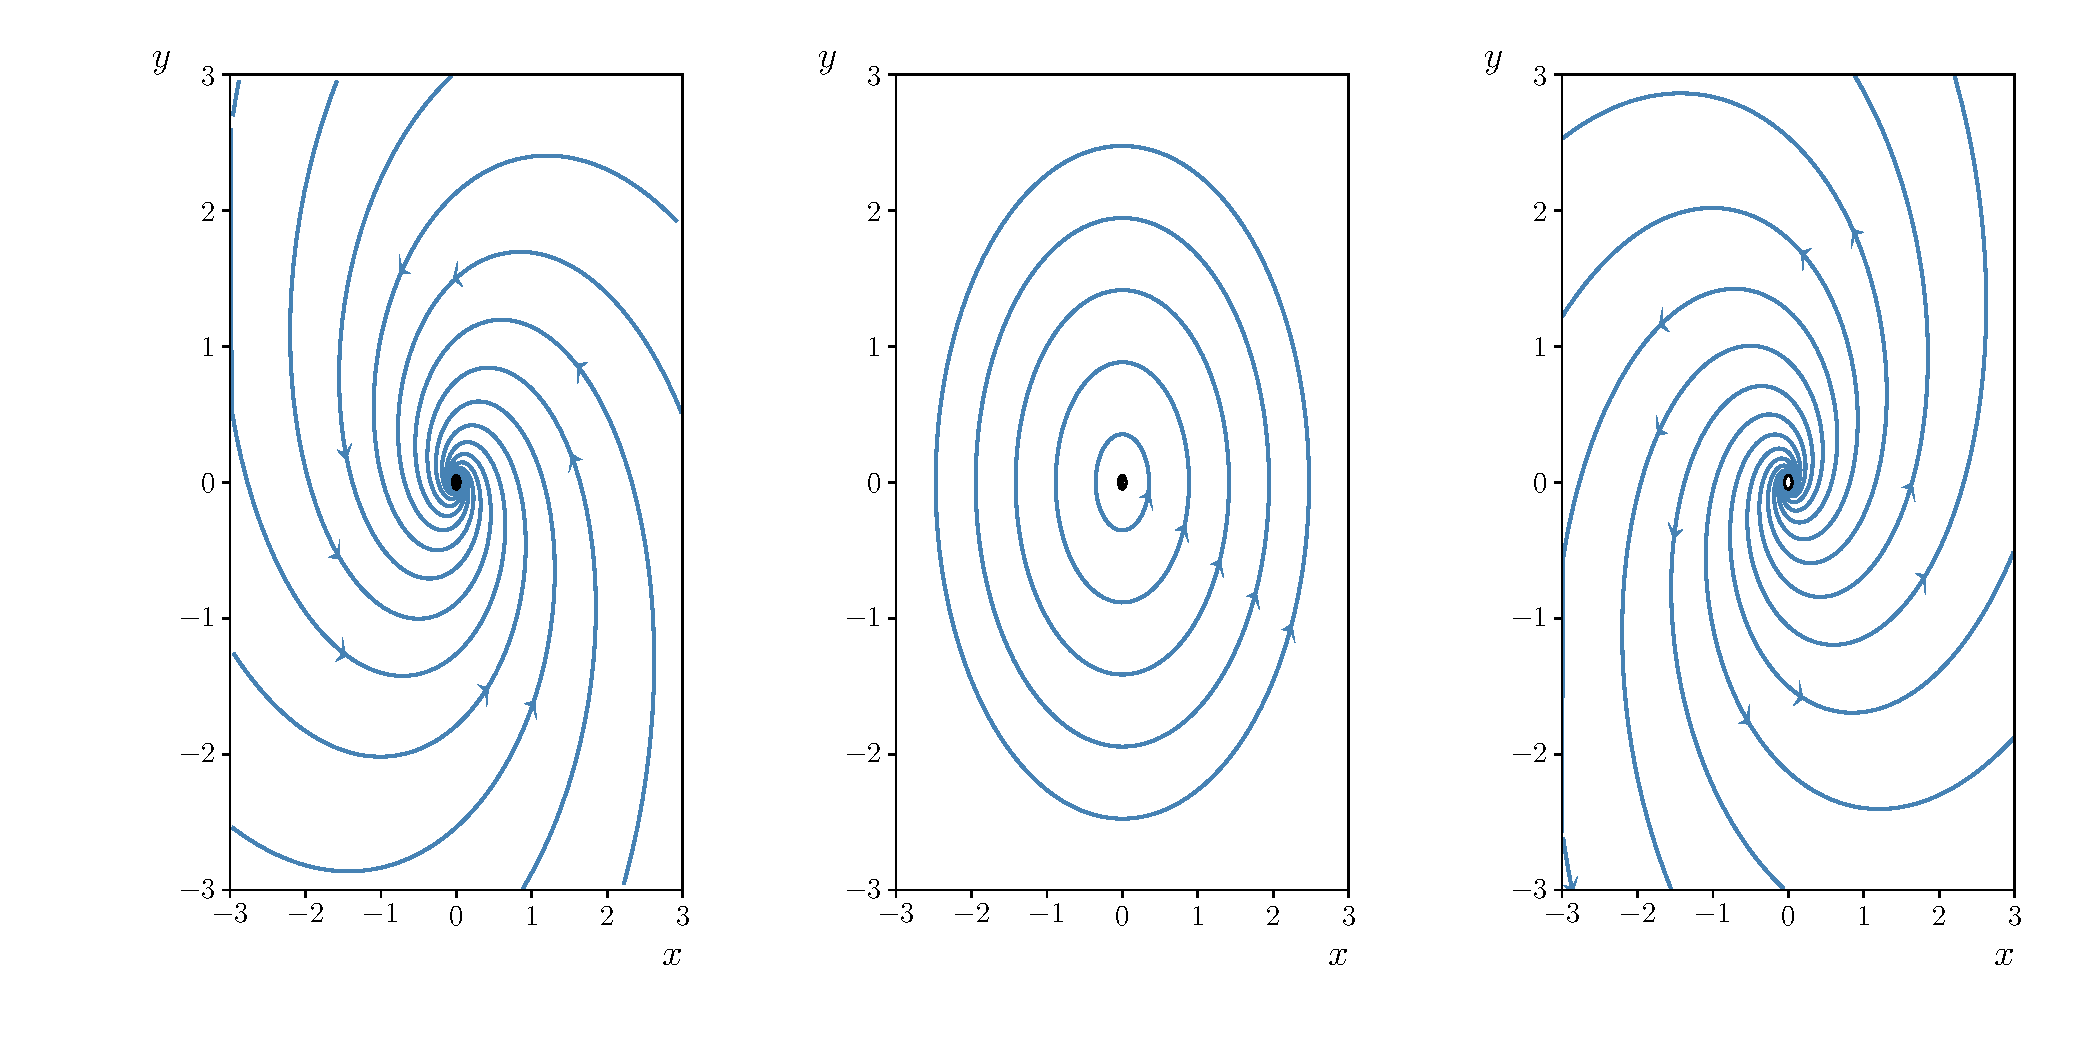
\includegraphics[scale= 0.6]{Q44_Phase_Portrait_All_Mu.eps}
	\caption{Phase portraits of the system for varying values of $\mu$ ($\omega = 1$ in all 
	cases).  From left to right $\lambda = -0.5$, $\lambda = 0$ and $\lambda = 0.5$. Attracting fixed points are denoted by filled circles, Liapunov stable by half-filled circles and 
	unstable by hollow circles.}
\end{figure}

\paragraph{}
It is useful to return to Polar form to consider the Poincare sections. Since all solutions to the 
DE rotate at a constant speed $\omega$, any surface which can be expressed as the set of all 
points with $r > 0$ and $\theta = C \in [0,2\pi)$ will be a valid Poincare section (assuming $\omega \neq 0$). 
Then since 

\begin{equation*}
	\Sigma = \left\{(r,\theta) \, | \, r>0, \, \theta = 0 \right\}
\end{equation*}

This surface is a valid Poincare section. However $\Sigma'$ is not a valid Poincare section as 
it includes the fixed point at the origin and at this point $F_p \cdot \nabla S(r,\theta) = 0$ 
for any surface $S$ by the definition of fixed points. Finally, since 

\begin{equation*}
	\Sigma_-'' = \left\{(r,\theta) \, | \, r> 0 \, \theta = \pi \right\}
\end{equation*}

is a valid Poincare section by the arguments above, it follows that $\Sigma \cup \Sigma_-'' = \Sigma''$ 
is also a valid Poincare section (these sections are disjoint and the transversality condition is 
satisfied on both pieces). So $\Sigma$ and $\Sigma''$ are valid Poincare sections but $\Sigma'$ is not.

\paragraph{}
Given solutions rotate with constant speed $\omega$ it is clear that, for a point $(x_n,y_n)$ on 
$\Sigma$, the solution will return to this surface after $2\pi/\omega$ units of time. Furthermore 
we know that $y = 0$ on both valid Poincare sections, so the first return map can be expressed 
concisely as

\begin{equation*}
	x_{n+1} = f(x_n) = x_ne^{\frac{2\lambda\pi}{\omega}}
\end{equation*}

By an identical argument, we can see that the time of first return for the surface $\Sigma''$ will 
be $\pi/\omega$ and so the first return map is

\begin{equation*}
	x_{n+1} = f(x_n) = -x_ne^{\frac{\lambda\pi}{\omega}}
\end{equation*}

\subsection*{Q44}
It is useful to convert this equation into polar coordinates using the same formulas as above. 
This leads to the differential equation $(\dot r, \dot \theta) = (r(1 - r^2),1)$. It is then 
clear that $x(t) = (\cos(t),\sin(t))$ (or $r = 1$, $\theta = t$) is a valid solution to this DE. 

\paragraph{}
We can then find the Floquet matrix (in Polar Coordinates) by solving the relevant part of the 
variational equations

\begin{equation*}
	\dot \Psi_t = DF(x(t))\Psi_t
\end{equation*}

Where $\Psi_t$ is the relevant Floquet matrix. Therefore, on the flow of interest we have 

\begin{equation*}
	\dot \Psi_t = 
	\begin{bmatrix}
		r - 3r^2 & 0 \\ 0 & 0
	\end{bmatrix}
	\biggr\rvert_{r = 1, \theta = t} \Psi_t \qquad \Psi_0 = I_2
\end{equation*}

Evaluating this we obtain the matrix DE

\begin{equation*}
	\dot \Psi_t = 
	\begin{bmatrix}
		-2 & 0 \\ 0 & 0
	\end{bmatrix} \Psi_t \qquad \Psi_0 = I_2
\end{equation*}

This can either be solved directly, or by noting that this is equivalent to the following system 
of equations 

\begin{align*}
	\dot a &= -2a \\ 
	\dot b &= 0 \\
	\dot c & = 0 \\
	\dot d &= 0 
\end{align*}

Where 

\begin{equation*}
	\Psi_t = 
	\begin{bmatrix}
		a & b \\ c & d
	\end{bmatrix}
\end{equation*}

Which leads naturally to the solution in Polar Coordinates 

\begin{equation*}
	\Psi_t = 
	\begin{bmatrix}
		e^{-2t} & 0 \\ 0 & 1
	\end{bmatrix}
\end{equation*}

To obtain the solution is cartesian coordinates, we will use the suggested notation provided 
and the definition of the Floquet matrix. Let $\varphi_t$ be the flow in cartesian coordinates 
and $\psi_t$ be the flow in polar coordinates. Let $r:(x,y) \rightarrow (r,\theta)$ be the 
polar coordinate transform and $\Phi_t$ the Floquet matrix in cartesian coordinates. Then by the definition of 
the Floquet matrix we have $\Phi_t = D\varphi_t = Dr^{-1}\circ \psi_t \circ r$. Applying the appropriate 
chain rule, this leads to the following expression for the Floquet matrix on the orbit of radius 
one (with initial condition $(x,y) = (1,0)$)

\begin{equation*}
	\Phi_t|_{(1,0)} = Dr^{-1}|_{\psi_t \circ r}\biggl\rvert_{(1,0)}\Psi_t|_r\biggl\rvert_{(1,0)}Dr\biggl\rvert_{(1,0)}
\end{equation*}

We can now evaluate each of these pieces in turn to obtain the solution. Given the function 
$r(x,y) = (\sqrt{x^2+y^2},\tan^{-1}(y/x))$ it is straightforward to obtain the linearization 

\begin{equation*}
	Dr|_{(1,0)} = 
	\begin{bmatrix}
		\frac{x}{\sqrt{x^2+y^2}} & \frac{y}{\sqrt{x^2+y^2}} \\ -\frac{y}{x^2+y^2} & \frac{x}{x^2+y^2}
	\end{bmatrix} \biggl \rvert_{(1,0)}
	= 
	\begin{bmatrix}
		1 & 0 \\ 0 & 1 
	\end{bmatrix}
	= I_2
\end{equation*}

Furthermore it is clear that $\Psi_t|_r\biggl\rvert_{(1,0)}$ is simply the Floquet matrix in Polar 
coordinates for this orbit, which we have calculated above. Finally we have 

\begin{equation*}
	Dr^{-1}|_{\psi_t \circ r}\biggl\rvert_{(1,0)} = (Dr)^{-1}|_{\varphi_t}\biggl\rvert_{(1,0)} = (Dr)^{-1}|_{x(t)}
\end{equation*}

Which can be computed directly as 

\begin{equation*}
	(Dr)^{-1}|_{x(t)} = 
	\begin{bmatrix}
		\cos(\theta) & -r\sin(\theta) \\ \sin(\theta) & r\cos(\theta)
	\end{bmatrix}^{-1}\biggr\rvert_{r=1,\,\theta = t}
	=
	\begin{bmatrix}
		\cos(t) & -\sin(t) \\ \sin(t) & \cos(t)
	\end{bmatrix}^{-1} 
	= 
	\begin{bmatrix}
		\cos(t) & -\sin(t) \\ \sin(t) & \cos(t)
	\end{bmatrix}
\end{equation*}

Combining these pieces, this leads to the desired result

\begin{equation*}
	\Phi_t = 
	\begin{bmatrix}
		\cos(t) & -\sin(t) \\ \sin(t) & \cos(t)
	\end{bmatrix}
	\begin{bmatrix}
		e^{-2t} & 0 \\ 0 & 1
	\end{bmatrix}
\end{equation*}

Then evaluating at $t = 2\pi$ this resolves to the matrix 

\begin{equation*}
	\Phi_{2\pi} = 
	\begin{bmatrix}
		e^{-4\pi} & 0 \\ 0 & 1
	\end{bmatrix}
\end{equation*}

The eigenvalues can be read directly from this matrix and are $e^{-4\pi} < 1$ and 1. The 
eigenvalue equivalence principle suggests that the first return map has one eigenvalue $e^{-4\pi}$ 
and so the periodic orbit is attracting.

\subsection*{Q47}
The fixed points of this system will occur at $x_* = 1 - ax_*^2 + y_*$, $y_* = bx_*$. Substituting 
the second equation into the first, we obtain a quadratic for $x_*$ so that 

\begin{equation*}
	x_* = \frac{(b-1) \pm \sqrt{(b-1)^2 + 4a}}{2a}
\end{equation*}

and obviously $y_* = bx_*$. Plugging in parameter values, this leads to 

\begin{equation*}
	x_* = \frac{-7 \pm \sqrt{609}}{28} \qquad y_* = \frac{3}{10}\left(\frac{-7 \pm \sqrt{609}}{28}\right)
\end{equation*}

The Jacobian at these points can be expressed as 

\begin{equation*}
	DF(x,y) = 
	\begin{bmatrix}
		-2ax_* & 1 \\ 0 & b
	\end{bmatrix} 
	=
	\begin{bmatrix}
		\frac{7 \mp \sqrt{609}}{10} & 1 \\ 0 & b
	\end{bmatrix}
\end{equation*}

The eigenvalues of this system can be obtained by the Trace-Determinant formula and are 

\begin{equation*}
	\lambda_{kj} = \frac{7 + (-1)^{k}\sqrt{609}}{20} + (-1)^j\sqrt{\frac{317}{10} + (-1)^k\frac{\sqrt{609}}{5}}
\end{equation*}

Where $\lambda_{kj}$ is the j-th eigenvalue of the k-th fixed point. We can calculate the 
eigenvalues for each fixed point as follows: for the fixed point at approximately $x = -1.1314$ 
(rounded to four significant figures) we have $\lambda_1 = 3.2598$ and $\lambda_2 = -0.0920$ 
(again rounded to four s.f.) with corresponding eigenvectors 

\begin{equation*}
	v_1 = 
	\begin{bmatrix}
		0.9958 \\ 0.0916
	\end{bmatrix}
	\qquad
	v_2 = 
	\begin{bmatrix}
		-0.2932 \\ 0.9560
	\end{bmatrix}
\end{equation*}

For the upper fixed point at approximately $x= 0.63135$ we have $\lambda_1 = -1.924$ 
and $\lambda_2 = 0.1560$ (all rounded to four s.f.). The corresponding eigenvalues are 

\begin{equation*}
	v_1 = 
	\begin{bmatrix}
		-0.9881 \\ 0.1541
	\end{bmatrix}
	\qquad 
	v_2 = 
	\begin{bmatrix}
		-0.4612 \\ -0.8872
	\end{bmatrix}
\end{equation*}

\paragraph{}
From this we can obtain the unstable subspaces for each point. The unstable subspace of the 
lower fixed point is $E^u = \{c(0.9958, 0.0916)\,|\, c \in \mathbb{R}\}$ and the unstable 
subspace at the upper fixed point is $E^u = \{c(-0.9881, 0.1541)\,|\,c \in \mathbb{R}\}$.

\paragraph{Finding the Unstable Manifold}
We can find a local approximation of the unstable manifold as the graph of a power series, 
centered on a fixed point $x_*$, $y_*$. We assume that local to a fixed point, we can write the 
unstable manifold as the graph of

\begin{equation*}
	y_* + h(x-x*) = y_* + a_0 + a_1(x-x_*) + a_2(x-x_*)^2 + \mathcal{O}(3)
\end{equation*}

Since this function must pass through the fixed point, we can assume $a_0 = 0$ safely. The invariance condition on this manifold (writing $\epsilon = x - x_*$)

\begin{equation*}
	(x_* + \epsilon',y_* + h(\epsilon')) = f(x_* + \epsilon, y + h(\epsilon))
\end{equation*}

Considering the second part of this equation first, we can see that this implies $y_* + bh(\epsilon') = bx_* + b\epsilon \implies h(\epsilon') = b\epsilon$. 
Furthermore, the first part implies that $x_* + \epsilon' = 1 - ax_*^2 - 2ax_*\epsilon - a\epsilon^2 + y_* + h(\epsilon) \implies \epsilon' = -2ax_*\epsilon - a\epsilon^2 + h(\epsilon)$. 
Substituting the first part into the second we obtain 

\begin{equation*}
	h(-2ax_*\epsilon - a\epsilon^2 + h(\epsilon)) = b\epsilon
\end{equation*}

Then expanding and gathering powers, we obtain the following recurrence relations for $a_1$ and $a_2$

\begin{align*}
	a_1(a_1 - 2ax_*) &= b \\
	a_1(a_2-a) + a_2(-2ax_* + a_1)^2 = 0
\end{align*}

Since this function must be tangent to the unstable subspace at the origin, we can obtain an 
expression for $a_1$ by approximating the slope from numerical eigenvalues we calculated above and thus do not need to solve 
the first recurrence relation. Solving the second recurrence relation, we obtain that 

\begin{equation*}
	a_2 = \frac{a_1a}{(a_1 - 2ax_*)^2 + a_1}
\end{equation*}

Substituting the appropriate values into these expressions, we obtain an estimate for the 
unstable manifold near each fixed point. At the lower fixed point at $-1.1314$ the unstable 
manifold is locally approximately described by the graph of the equation $y = y_* + h(x-x_*) =  0.0920(x-x_*) + 0.0120(x-x_*)^2$ 
and at the upper fixed point the unstable manifold is locally approximately described by 
$y = y_* + h(x-x_*) = -0.1559(x-x_*) - 0.0616(x-x_*)^2$.

\paragraph{}
By choosing a small set of points within this unstable manifold and iterating forward, we can 
obtain a sketch of at least a portion of the unstable manifold (\autoref{fig:henon_map}).

\begin{figure}[H]
    \centering
	\hspace{-0.5in}
    \includegraphics[scale = 0.5]{Henon_Map_Unstable_Manifold.png}
	\caption{A sketch of the Henon map's unstable manifold, generated by 20 forward iterations of 
	points on the local estimates of the unstable manifolds.}
    \label{fig:henon_map}
\end{figure}

\subsection*{2021 Exam Question 4}
\paragraph{(a)}
Given the system $\nabla(x,y) = (x^2+xy -y^2,\mu x - y)$ it is straightforward to see that there 
is a fixed point at the origin. The Jacobian evaluated at this point is 

\begin{equation*}
	DF = 
	\begin{bmatrix}
		0 & -1 \\
		\mu & -1
	\end{bmatrix}
\end{equation*}

So one eigenvalue of this matrix is clearly $\mu$. Therefore this system must experience a 
bifurcation at $\mu =0$ as one eigenvalue passes through zero at this point. Consequently, we wish to find the center manifold. Therefore 
we linearize the extended system (including $\dot \mu = 0$) to obtain 

\begin{equation*}
	DF = 
	\begin{bmatrix}
		2x+y & x-2y-1 & 0 \\ \mu & -1 & 0 \\ 0 & 0 & 0 
	\end{bmatrix}
\end{equation*}

Evaluating this at the fixed point we obtain the Jacobian of the extended system 

\begin{equation*}
	DF = 
	\begin{bmatrix}
		0 & -1 & 0 \\ 0 & -1 & 0 \\ 0 & 0 & 0 
	\end{bmatrix}
\end{equation*}

This has one stable direction, so $E_s = span\{e_1 + e_2\}$ (where $e_i$ is the i-th standard 
basis vector) and the center subspace is $E_c = span\{e_1,\, e_3\}$. We will assume that 
there exists a function $h(x,\mu)$ such that graph of $y = h(x,\mu)$ is equal to the center 
manifold (at least for small $x$, $\mu$). This implies that this surface must be tangent to the 
center subspace at the origin, or, equivalently, that the normal vectors to this surface must 
be orthogonal to the center subspace. This implies that $\nabla(y-h(x,\mu)) \in span\{e_2\}$ 
and so a power series expansion of $h$ must not contain any terms of order one. Furthermore, since 
$h$ must pass through the origin it must also not contain any terms of order zero. Therefore, 
a power series expansion of $h$ must be of the form

\begin{equation*}
	h(x,\mu) = ax^2 + bx\mu + c\mu^2 + \mathcal{O}(3)
\end{equation*}

As required.

\paragraph{(b)}
The invariance condition for $h$ is simply $\dot y = h_x \dot x + h_\mu \dot \mu$, which is 
further simplified when one recalls that $\dot \mu = 0$. Therefore we require that 

\begin{equation*}
	\mu x - h(x,\mu) = (2ax + b\mu + \mathcal{O}(2))(x^2 - h(x,\mu) + xh(x,\mu) - (h(x,\mu))^2)
\end{equation*}

Expanding $h$ and gathering like orders we obtain that

\begin{align*}
	\mathcal{O}(0): &\quad 0 = 0 \\
	\mathcal{O}(1): &\quad 0 = 0 \\
	\mathcal{O}(2): &\quad \mu x - ax^2 - b\mu x - c\mu^2 = 0 \\
\end{align*}

The further requirement that terms of each order must be balanced in powers of both $x$ and $\mu$ 
clearly requires that $a = 0$, $b=1$ and $c=0$. Therefore the local approximation of $h$ is given 
by 

\begin{equation*}
	h(x,\mu) = \mu x + \mathcal{O}(3)
\end{equation*}

\paragraph{(c)}
Substituting in the truncated center manifold in place of $y$, we find that near the origin the 
dynamics on the center manifold are well-approximated by 

\begin{align*}
	\dot x &= x^2 - \mu x + \mu x^2 - \mu^2 x^2 \\
	\dot y &= 0 \\
	\dot \mu &= 0
\end{align*}

So the system can be locally reduced to a one-dimensional problem on the center manifold. 
The fixed points on this manifold are $x = 0$ and $x = \mu/(1+\mu-\mu^2)$. Furthermore, we 
can find $\ddot x = -\mu + 2x(1+\mu-\mu^2)$. This one-dimensional problem can now be analyzed 
using linear stability theory, which shows that the fixed point at the origin is unstable for 
$\mu < 0$ and stable for $\mu > 0$, while the other fixed point is stable for $\mu < 0$ and 
unstable for $\mu > 0$. Since at $\mu = 0$ the two fixed points are equal, this suggests a 
transcritical bifurcation occurs when $\mu = 0$. 

\paragraph{(d)}
\begin{figure}
	\hspace{-0.6in}
	\includegraphics[scale=0.5]{Exam_Q_Phase_Portrait_Neg_Mu.eps}
	\includegraphics[scale=0.5]{Exam_Q_Phase_Portrait_Mid_Mu.eps}
	\vspace{-0.05in}
	\begin{center}
	\includegraphics[scale=0.5]{Exam_Q_Phase_Portrait_Large_Mu.eps}
	\end{center}
	\caption{Phase portraits of the system near the fixed points and varying values of $\mu$. 
	From right to left: $\mu < 0$, $\mu = 0$, $\mu > 0$. Stable fixed points are 
	denoted by filled black circles, unstable by hollow circles and half-stable by half-filled 
	circles.}
    \label{fig:exam_phase portraits}
\end{figure}

\end{document}
